%&preformat-disser
\RequirePackage[l2tabu,orthodox]{nag} % Раскомментировав, можно в логе получать рекомендации относительно правильного использования пакетов и предупреждения об устаревших и нерекомендуемых пакетах
% Формат А4, 14pt (ГОСТ Р 7.0.11-2011, 5.3.6)
\documentclass[a4paper,14pt,oneside,openany]{memoir}

\input{common/setup}            % общие настройки шаблона
\input{common/packages}         % Пакеты общие для диссертации и автореферата
\synopsisfalse                      % Этот документ --- не автореферат
\input{Dissertation/dispackages}    % Пакеты для диссертации
\input{Dissertation/userpackages}   % Пакеты для специфических пользовательских задач

\input{Dissertation/setup}      % Упрощённые настройки шаблона

\input{common/newnames}         % Новые переменные, для всего проекта

\input{common/data}             % Основные сведения
\input{common/fonts}            % Определение шрифтов (частичное)
\input{common/styles}           % Стили общие для диссертации и автореферата
\input{Dissertation/disstyles}  % Стили для диссертации
\input{Dissertation/userstyles} % Стили для специфических пользовательских задач

%%% Библиография. Выбор движка для реализации %%%
% Здесь только проверка установленного ключа. Сама настройка выбора движка
% размещена в common/setup.tex
\ifnumequal{\value{bibliosel}}{0}{%
    \input{biblio/predefined}   % Встроенная реализация с загрузкой файла через движок bibtex8
}{
    \input{biblio/biblatex}     % Реализация пакетом biblatex через движок biber
}

% Вывести информацию о выбранных опциях в лог сборки
\typeout{Selected options:}
\typeout{Draft mode: \arabic{draft}}
\typeout{Font: \arabic{fontfamily}}
\typeout{AltFont: \arabic{usealtfont}}
\typeout{Bibliography backend: \arabic{bibliosel}}
\typeout{Precompile images: \arabic{imgprecompile}}
% Вывести информацию о версиях используемых библиотек в лог сборки
\listfiles

%%% Управление компиляцией отдельных частей диссертации %%%
% Необходимо сначала иметь полностью скомпилированный документ, чтобы все
% промежуточные файлы были в наличии
% Затем, для вывода отдельных частей можно воспользоваться командой \includeonly
% Ниже примеры использования команды:
%
%\includeonly{Dissertation/part2}
%\includeonly{Dissertation/contents,Dissertation/appendix,Dissertation/conclusion}
%
% Если все команды закомментированы, то документ будет выведен в PDF файл полностью

\begin{document}
%%% Переопределение именований типовых разделов
% https://tex.stackexchange.com/a/156050
\gappto\captionsrussian{\input{common/renames}\unskip} % for polyglossia and babel
\input{common/renames}

%%% Структура диссертации (ГОСТ Р 7.0.11-2011, 4)
% Титульный лист (ГОСТ Р 7.0.11-2001, 5.1)
\thispagestyle{empty}
\begin{center}
	Федеральное государственное автономное образовательное учреждение высшего образования «Дальневосточный федеральный университет»
\end{center}
%
\vspace{0pt plus4fill} %число перед fill = кратность относительно некоторого расстояния fill, кусками которого заполнены пустые места
\IfFileExists{images/FEFU_logo.eps}{
	\begin{minipage}[b]{0.5\linewidth}
		\begin{flushleft}
			\includegraphics[height=3.5cm]{FEFU_logo}
		\end{flushleft}
	\end{minipage}%
	\begin{minipage}[b]{0.5\linewidth}
		\begin{flushright}
			На правах рукописи\\
			%      \textsl {УДК \thesisUdk}
		\end{flushright}
	\end{minipage}
}{
	\begin{flushright}
		На правах рукописи
		
		%\textsl {УДК \thesisUdk}
	\end{flushright}
}
%
\vspace{0pt plus6fill} %число перед fill = кратность относительно некоторого расстояния fill, кусками которого заполнены пустые места
\begin{center}
	{\large Трухин Вячеслав Олегович}
\end{center}
%
\vspace{0pt plus1fill} %число перед fill = кратность относительно некоторого расстояния fill, кусками которого заполнены пустые места
\begin{center}
	\textbf {\large %\MakeUppercase
		Статистическая механика векторных моделей с фрустрациями}
	
	\vspace{0pt plus2fill} %число перед fill = кратность относительно некоторого расстояния fill, кусками которого заполнены пустые места
	{%\small
		Специальность 01.06.03\ "---
		
		<<Физика и астрономия>>
	}
	
	\ifdefined\thesisSpecialtyTwoNumber
	{%\small
		Специальность \thesisSpecialtyTwoNumber\ "---
		
		<<\thesisSpecialtyTwoTitle>>
	}
	\fi
	
	\vspace{0pt plus2fill} %число перед fill = кратность относительно некоторого расстояния fill, кусками которого заполнены пустые места
	Выпускная квалификационная работа
\end{center}
%
\vspace{0pt plus4fill} %число перед fill = кратность относительно некоторого расстояния fill, кусками которого заполнены пустые места
\begin{flushright}
	\ifdefined\supervisorTwoFio
	Научные руководители:
	
	\supervisorRegalia
	
	\ifdefined\supervisorDead
	\framebox{\supervisorFio}
	\else
	\supervisorFio
	\fi
	
	\supervisorTwoRegalia
	
	\ifdefined\supervisorTwoDead
	\framebox{\supervisorTwoFio}
	\else
	\supervisorTwoFio
	\fi
	\else
	Научный руководитель:
	
	доктор ф.-м. наук, профессор
	
	\ifdefined\supervisorDead
	\framebox{\supervisorFio}
	\else
	Нефедев Константин Валентинович
	\fi
	\fi
	
\end{flushright}
%
\vspace{0pt plus4fill} %число перед fill = кратность относительно некоторого расстояния fill, кусками которого заполнены пустые места
{\centering Владивосток\ "--- \thesisYear\par}
           % Титульный лист
\include{Dissertation/contents}        % Оглавление
\ifnumequal{\value{contnumfig}}{1}{}{\counterwithout{figure}{chapter}}
\ifnumequal{\value{contnumtab}}{1}{}{\counterwithout{table}{chapter}}
\chapter*{Введение}                         % Заголовок
\addcontentsline{toc}{chapter}{Введение}    % Добавляем его в оглавление

\newcommand{\actuality}{}
\newcommand{\progress}{}
\newcommand{\aim}{{\textbf\aimTXT}}
\newcommand{\tasks}{\textbf{\tasksTXT}}
\newcommand{\novelty}{\textbf{\noveltyTXT}}
\newcommand{\influence}{\textbf{\influenceTXT}}
\newcommand{\methods}{\textbf{\methodsTXT}}
\newcommand{\defpositions}{\textbf{\defpositionsTXT}}
\newcommand{\reliability}{\textbf{\reliabilityTXT}}
\newcommand{\probation}{\textbf{\probationTXT}}
\newcommand{\contribution}{\textbf{\contributionTXT}}
\newcommand{\publications}{\textbf{\publicationsTXT}}


{\actuality} Фазовые переходы в системах конечного числа частиц чрезвычайно широко распространены в естественной природе, и не представляет труда найти множество примеров таких превращений. Например, стоит вспомнить таяние крохотной снежинки и превращение ее в капельку воды, для фазового перехода первого рода в системе конечного числа атомов, или же спонтанное возникновение магнитного момента у однодоменной наночастицы, в случае фазового перехода второго рода. 

Наличие теоретической или экспериментальной фазовой диаграммы для конкретной модели обычно означает завершенность теории и глубокий уровень нашего понимания природы явлений в системах многих взаимодействующих тел. Одной из самых простых моделей взаимодействующих многих тел является модель Изинга. Оказалось, не смотря на более чем вековую историю исследования этой самой простой модели c взаимодействием ближайших соседей из первой координационной сферы, даже в самом простом случае, в отсутствии внешнего магнитного поля, оказывается не так просто с помощью таких мощных и зарекомендовавших себя в теоретической физике методов, построить теоретическую магнитную фазовую диаграмму, например, в осях ''Температура---Вероятность'', $T(P_+)$. Под температурой $T$ мы понимаем критическую температуру фазового превращения, под вероятностью $P_+$ понимаем вероятность того, что случайно взятая пара взаимодействующих спинов имеет ферромагнитную связь $+J$, т.е. значение обменной константы $J>0$. Очевидно, что для ферромагнетика $P_+=1$, для антиферромагнетика $P_+=0$, для спинового стекла $P_+=0.5$.

Подходы к завершению теории, т.е. к построению фазовой диаграммы продолжаются и с помощью аналитических методов \cite{belokon2006}, численными Монте-Карло расчетами \cite{Hasenbusch2008}, и экспериментально \cite{Mirebeau2022}. Как будет показано ниже прямые строгие вычисления статистической суммы в модели Изинга для конечного числа взаимодействующих частиц позволяют решить множество задач без привлечения методов теории нарушения симметрии реплик (RSB) \cite{newman2023proof}.

В данной работе мы вычислили границы между ферромагнитным, парамагнитным, спинстекольным и антиферромагнитным состояниями. Эдвардс и Андерсон показали, что в таких магнетиках возможен новый тип фазового перехода, который связан с замораживанием спинов \cite{edwards1975theory}. В работах \cite{Ground2010pmJ, Correlation2005SG} модель Эдвардса-Андерсона (ЭА) определяется как модель с бимодальным распределением обменных интегралов. Модуль обменного интеграла $J$ принимает одинаковые значения для всех взаимодействий между спинами в ближайшем окружении. В модели ЭА обменная константа $J$ может принимать только два возможных значения ''+1'' или ''-1''. 

В работах \cite{Feigelman1985Hierarchical, Murani1977Spin, Deryabin1983Features} ЭА-модель применяется для описания результатов экспериментов с $FeAu$, $FeNiMn$, $PtMnFe$ при отличных от нуля температурах.  Таких проявлений частично неупорядоченной или неупорядоченной конденсированной материи очень много в реальной природе, наверное даже много больше, чем теоретических моделей таких состояний \cite{ziman1979models}. В распоряжении теоретика имеется только небольшое число точно решаемых теоретических моделей \cite{baxter2016exactly}, которые разрабатывались для понимания структуры, различных свойств и в целом природы материи \cite{ziman1979models}. На исследование состояния спинового стекла было потрачено множество усилий \cite{binder1986spin, fischer1993spin, young1998spin, bezzub1983}. Модель спинового стекла с конечным радиусом взаимодействия оказалась сложной задачей для систем бесконечного числа частиц \cite{kor1989}. Некоторые теоретические вопросы до сих пор остаются открытыми для моделей бесконечного радиуса\cite{sherrington1975solvable}. Предпринимались попытки получить решение в модели конечного радиуса также и методами среднего поля \cite{belokon2006, belokon2001funk}. 

В данной работе методами Монте-Карло и исчерпывающего перечисления для конечного числа спинов Изинга в модели ограниченного радиуса (ближайших соседей) приближенно для образцов относительно большого числа частиц $N=40\times40$ и строго для малого числа частиц $N=8\times8$, получены критические температуры для заданного среднего значения обменной константы $P_+$. Точное решение позволило вычислить статистические суммы для систем конечного числа спинов в модели Изинга с отрытыми граничными условиями. Мы использовали результаты, приведенные в работе \cite{makarov2019} для численного расчета параметра фрустраций исследуемых моделей. Все это позволило построить теоретические фазовые магнитные диаграммы для ферромагнитной фазы, антиферромагнитной фазы и спинового стекла, в том числе и во внешнем магнитном поле.
 % Характеристика работы по структуре во введении и в автореферате не отличается (ГОСТ Р 7.0.11, пункты 5.3.1 и 9.2.1), потому её загружаем из одного и того же внешнего файла, предварительно задав форму выделения некоторым параметрам

%\textbf{Объем и структура работы.} Диссертация состоит из~введения,
%\formbytotal{totalchapter}{глав}{ы}{}{},
%заключения и
%\formbytotal{totalappendix}{приложен}{ия}{ий}{}.

%% на случай ошибок оставляю исходный кусок на месте, закомментированным
%Полный объём диссертации составляет  \ref*{TotPages}~страницу
%с~\totalfigures{}~рисунками и~\totaltables{}~таблицами. Список литературы
%содержит \total{citenum}~наименований.
%

%Полный объём диссертации составляет
%\formbytotal{TotPages}{страниц}{у}{ы}{}, включая
%\formbytotal{totalcount@figure}{рисун}{ок}{ка}{ков} и
%\formbytotal{totalcount@table}{таблиц}{у}{ы}{}.
%Список литературы содержит
%\formbytotal{citenum}{наименован}{ие}{ия}{ий}.
    % Введение
\ifnumequal{\value{contnumfig}}{1}{\counterwithout{figure}{chapter}
}{\counterwithin{figure}{chapter}}
\ifnumequal{\value{contnumtab}}{1}{\counterwithout{table}{chapter}
}{\counterwithin{table}{chapter}}
\chapter{Модель}\label{ch:ch1}

\section{Модель Изинга на простой квадратной решетке}
Модель Изинга использовалась для исследования условий существования ферромагнетизма, антиферромагнетизма и спинового стекла. Эти термодинамические состояния могли быть обнаружены для исследуемых систем ниже найденных нами критических температур в зависимости от знака обменной константы взаимодействующих со своими ближайшими соседями $N$ спинов Изинга $S_i$, расположенных в узлах квадратной решетки. Ферромагнитные взаимодействия $J_{ij}=+1$ и антиферромагнитные взаимодействия $J_{ij}=-1$ случайным образом равномерно были распределены для всех $ij$-пар взаимодействующих спинов с заданной вероятность $P_+$. Энергия взаимодействия рассчитывалась по правилу
\begin{equation}
	E_t = -\sum_{<ij>}J_{ij} S_iS_j-HM_i,
	\label{eq:internal_energy}
\end{equation}
где $<ij>$ означает, что суммирование происходит только по ближайшим соседям, $H$ -- внешнее магнитное поле.  Спиновый избыток
\begin{equation}
	M_i = \sum_{j=1}^NS_j.
	\label{eq:spinex}
\end{equation}

Для каждого спинового избытка может существовать несколько различных значений энергии $E_t$, каждое со своим вырождением $g_t$. С учетом внешнего магнитного поля $H$ статсумма равна

\begin{equation}  
	Z=\sum_{l=1}^{2^N}\exp\left\{-\frac{E_l}{kT}\right\}=\sum_{t=1}^{\Omega}g_t \exp\left\{-\frac{E_t}{kT}\right\},
	\label{eq:partfunk}
\end{equation}
где $\Omega$ --- это общее число вырожденных состояний со всеми возможными значениями спинового избытка $M_i$, $k=1$ --- постоянная Больцмана.            % Глава 1
\chapter{Методы расчёта}\label{ch:ch2}

\section{Методы расчёта критических температур для систем конечного числа спинов Изинга} Для строгого расчета теоретической фазовой диаграммы $T(P_+)$ были рассчитаны строго статистические суммы для десяти образцов со случайным равномерным распределением обменных констант по всем парам взаимодействующих спинов, а также выполняли Монте-Карло расчеты для такого же количества образцов. Необходимо отметить, что строгий расчет статистической суммы в модели Изинга для систем произвольного числа взаимодействующих спинов $N$ со случайным распределением обменных интегралов во внешнем магнитном поле представляет собой сложную задачу, для которой сегодня отсутствуют алгоритмы численного расчета, время работы которых полиномиально зависит от числа спинов $N$. Чтобы рассчитать статистическую сумму необходимо выполнить расчет энергии всех $2^N$ конфигураций в ходе исчерпывающего перечисления, т.е. существующие алгоритмы являются экспоненциально длительными.

Был разработан параллельный алгоритм (алг. \ref{algo:dos_exhaustive}), позволивший получить распределение Гиббса в модели конечного числа спинов (до $8\times8$)  с взаимодействием ближайших соседей на квадратной решетке со свободными граничными условиями. Метод исчерпывающего перечисления был использован в авторском параллельном суперкомпьютерном коде, с помощью которого проведены численные расчеты. Проводилась декомпозиция системы на элементы (одномерные цепочки). Плотное побитовое кодирование позволило хранить информацию (энергию, спиновый избыток, вырождение и др.) обо всех конфигурации подсистем из двух одномерных решёток спинов с учетом распределения обменных интегралов в подсистемах.  Энергия двух объединенных одномерных решеток в двумерную или присоединение одномерной решетки к двумерной будет следующей:
\begin{equation}
	E_{sum}  = E_{l}  + E_{r}  + E_{u},
	\label{eq:unification_energy}
\end{equation}

\noindent где $E_{l}$, $E_{r}$ -- энергии левой и правой решетки соответственно, $E_{u}$ энергия объединения решёток. 

Библиотека состояний подсистем позволяет значительно масштабировать число частиц. Мы использовали четное число спинов в системе $8\times8$, чтобы статистическая сумма содержала конфигурации с нулевым спиновым избытком для исключения влияния некомпенсированного спинового избытка на расчет термодинамических свойств во внешнем магнитном поле.

Основные положения метода Монте-Карло при расчете с помощью алгоритма Метрополиса, а также описание численного расчета термодинамических средних как для систем, где обменная энергия зависит от расстояния, так и для моделей ограниченного радиуса можно, например, найти, например, в серии наших работ  \cite{Shevchenko2017, makarov2019, Shevchenko2022, makarova2023}. Мы использовали следующие основные параметры алгоритма Метрополиса для расчета образцов $N=40\times40$ с заданным распределением обменных констант: количество шагов Монте-Карло составляло $10^5$ для приведения системы спинов в равновесное состояние; количество шагов для усреднения энергии и поиска кандидата на основное состояние выбиралось $10^6$; усреднение проводилось по всем полученным в ходе Монте-Карло семплирования конфигурациям, каждая из которых имела свое значение энергии.

\section{Алгоритм и особенности реализации}

Для строгого расчёта статистической суммы образов с заданным $P_+$ имитирующих ферромагнетик, антиферромагнетик и спиновое стекло был разработан параллельный высокопроизводительный алгоритм, который в последствии был реализован на языке CUDA.

!!!!Здесь будет псевдокод но он не вставляется!!!!

%\begin{algorithm}[H]
%	\textbf{INPUT:} Cell size, exchange integral distribution.\\
%	\textbf{OUTPUT:} Full density of states.
%	\begin{algorithmic}
%		\STATE {GPU configuration:}
%		\STATE {creating massive of configurations 1D chain by bit offset}
%		\STATE {creating G-tensor [config right][E][M][prime number set]}
%		\FOR {Number of layer in cell\\}
%		{
%			\FOR {Each added 1D chain\\}
%			{
%				\FOR {Each configuration of the outermost layer of the build-up lattice\\}
%				{
%					\FOR{Each configuration of added 1D chain\\}
%					\STATE {Calculate energy and magnetic susceptibility}
%					\STATE {Atomic add degeneration of the build-up lattice in G-tensor[configuration of outermost layer][energy][magnetic susceptibility][prime numer coefficients]}
%					\ENDFOR\\
%				}
%				\ENDFOR\\
%			}
%			\ENDFOR
%		}
%		\ENDFOR
%		\STATE{Deciphering degeneracies from the set of prime numbers}
%		\STATE{Reformating data from G-tensor to degeneracy, energy, magnetic susceptibility density of states}
%	\end{algorithmic}
%	\caption{Calculation density of states by exhaustive search.}
%	\label{algo:dos_exhaustive}
%\end{algorithm}

В расчетах на GPU узким местом является запись и чтение в global память, и, чтобы не тратить время на многократную запись накапливающихся в результате вычислений данных о вырождении, энергии и спиновом избытке  был создан массив G-tensor [config right][E][M][prime number set] с осями размера одномерной цепочки, максимальной энергии $\times 2 + 1$, максимального спинового избытка $\times 2 + 1$ и набор простых чисел для записи вырождения, соответственно. В этот тензор в процессе расчёта атомарно добавлялась информация о вырождении по координатам энергии $+ E_{max}$ и спинового избытка $+ M_{max}$.

Координата конфигурации цепочки была нужна для то чтобы знать какую конфигурацию правого слоя мы соединяем с новой 1D цепочкой справа и какие состояния всей левой решетки с этой конфигурацией связаны.

Поскольку вырождение состояний с одинаковой энергией и спиновым избытком могут принимать значения от $1$ до $\approx 2^{N}$, где $N$ -- размер решетки, то при размерах больше чем $8 \times 8$ вырождения уже не помещаются в целочисленный встроенный тип. Для решения этой проблемы получаемые при решении вырождения разбиваются на простые числа, а после всех расчётов расшифровываются с помощью китайской теоремы об остатках \cite{katz2007mathematics}.           % Глава 2
\chapter{Фазовая диаграмма}\label{ch:ch3}

\section{Теоретическая магнитная фазовая диаграмма в отсутствии поля} Каждый образец содержал долю $P_{+}$ ферромагнитных связей  $J_{ij}=+1$. Все взаимодействия были только антиферромагнитными $J_{ij}=-1$, если $P_{+}=0$. Для каждой концентрации $P_{+}$ было получено по десять образцов со случайным равномерным распределением $J_{ij}$. 

Границы фаз или критические температуры переходов ''ферромагнетизм-спиновое стекло''  и ''антиферромагнетизм-спиновое стекло'' $T(P_{+})$ получены приближенно, как температуры точек перегиба параметра фрустраций \cite{makarov2019} 

\begin{equation}
	F_p(T) = \frac{E_{max} + \langle E \rangle (T)}{2E_{max}},
	\label{eq:frustration_parameter}
\end{equation}
см. рисунок \ref{fig:fp0}. 

\begin{figure}[!ht]
	\centering
	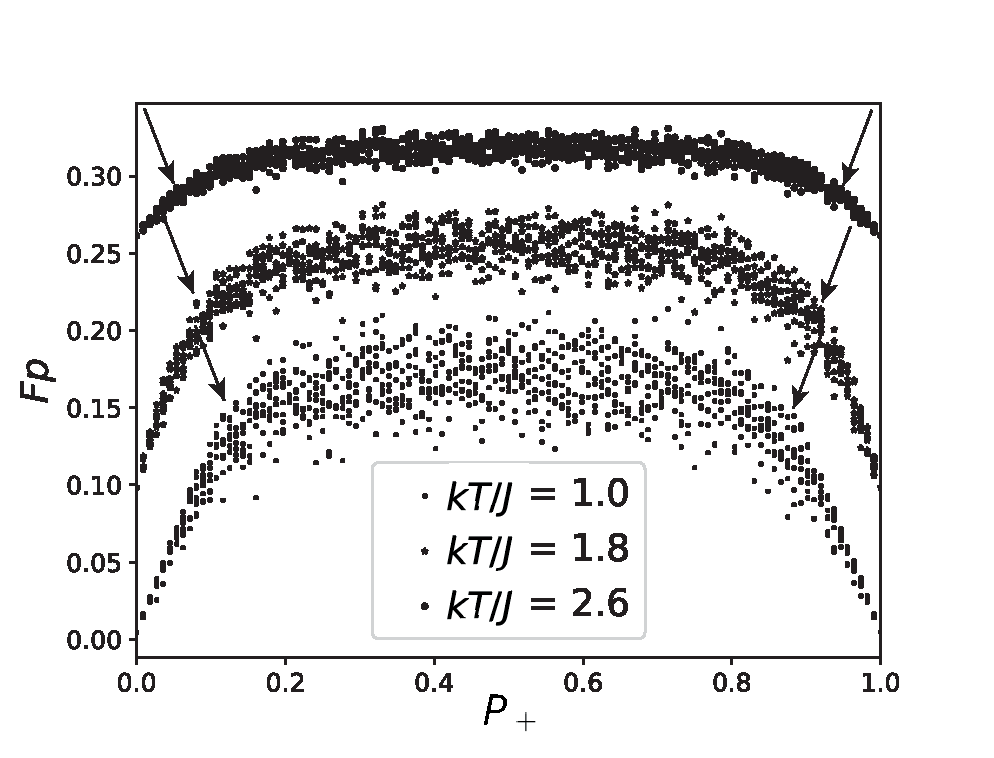
\includegraphics[width=0.7\linewidth]{Frustration_parameter_h0.0.eps}
	\caption{Зависимость параметра фрустрации от концентрации $P_{+}$ обменных констант для образцов $N=8\times8$ без внешнего поля для температур, указанных на вставке}
	\label{fig:fp0}
\end{figure}

Максимальная энергия системы $E_{max}$ --- сумма по модулю всех парных энергий взаимодействия. В отличном от нуля поле энергия Зеемана добавляется в виде слагаемого с максимальным спиновым избытком

\begin{equation}
	E_{max} = 2NJ_{ij}(N-1) + MH, \quad M = N.
	\label{eq:Emax}
\end{equation}

Граница фаз ''парамагнетик-спиновое стекло'' определена путем численных расчетов температуры максимума теплоемкости $C_{max}(T)$ в температурной зависимости
\begin{equation}
	C(T)=\frac{\partial \langle E \rangle (T)}{\partial T}=\frac{\langle E^2 \rangle-\langle E \rangle ^2}{k T^2},
	\label{eq:ct}
\end{equation}
где
\begin{equation}
	\langle E \rangle (T) =\frac{1}{Z}\sum_{t=1}^{\Omega}g_t E_t \exp\left\{-\frac{E_t}{kT}\right\}
	\label{eq:ct}
\end{equation}
и
\begin{equation}
	\langle E^2 \rangle (T) =\frac{1}{Z}\sum_{t=1}^{\Omega}g_t E_t^2 \exp\left\{-\frac{E_t}{kT}\right\}.
	\label{eq:ct}
\end{equation}

На рисунке \ref{fig:Diag} представлена теоретическая магнитная фазовая диаграмма, где PM --- парамагнетизм, SG --- спиновое стекло, FM --- ферромагнетизм и AFM -- антиферромагнетизм. Звездочками обозначены критические температуры точек перегиба параметра фрустраций $T(P_{+})$, или критические температуры фазового превращения, крестами -- критические значения температур теплоёмкости, круглыми синими точками обозначены критические температуры наступления ферромагнетизма. Такие же обозначения использованы на рисунках \ref{fig:Diag1} и \ref{fig:Diag4}.

\begin{figure}[!ht]
	\centering
	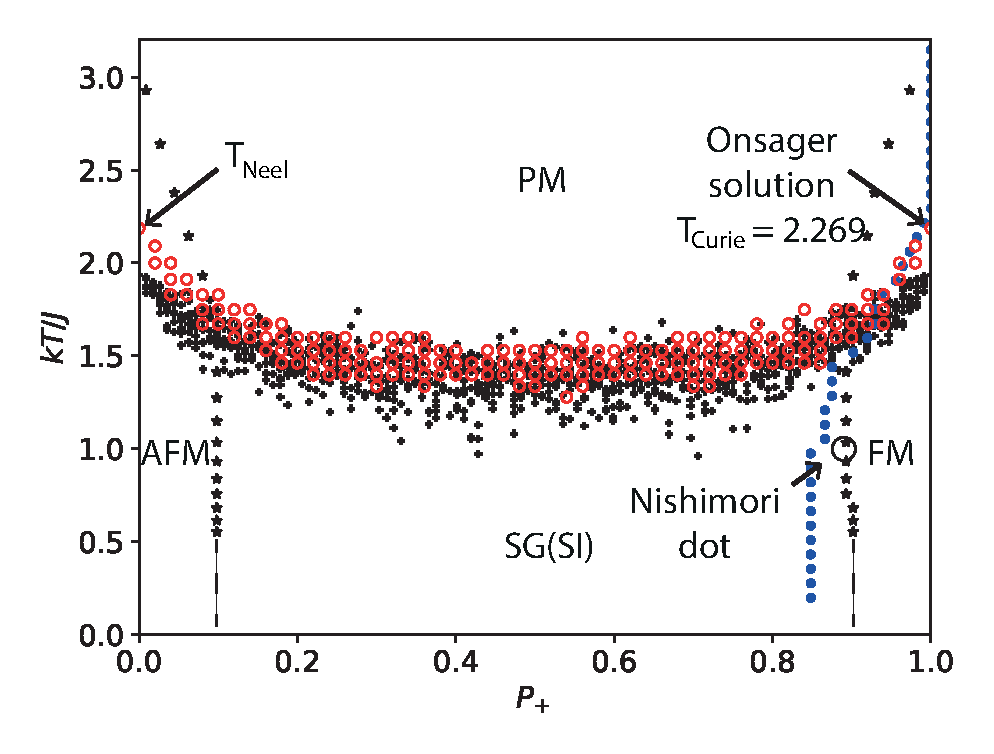
\includegraphics[width=0.8\linewidth]{Phase_diagram_h0_with_vashche_all.eps}
	\caption{Теоретическая магнитная фазовая диаграмма в отсутствии внешнего магнитного поля. Черные крестики --- точный расчет температуры максимума теплоемкости, красные пустые кружочки --- температура максимума теплоемкости, рассчитанная методом Метрополиса, синие заполненные кружочки ---  рассчитанные значения модуля намагниченности, звездочки --- результаты получены по перегибу параметра порядка.}
	\label{fig:Diag}
\end{figure}

Круглые точки получены следующим образом: считалась вероятность ферромагнетизма по заданному значению модуля спинового избытка (\ref{eq:P_M}) при определенной температуре, затем находилась конфигурация, при которой вероятность ферромагнетизма $P(FM)$ становится меньше $0.95$ и ставилась точка на график (рис. \ref{fig:Diag}).

\begin{equation}
	P(E_{gs}) =\frac{g_{gs}}{Z} \exp\left\{-\frac{E_{gs}}{kT}\right\},
	\label{eq:P_M}
\end{equation}
при этом для спинового избытка основного состояния $M_{gs}$ выполнялось неравенство

\begin{equation}
	\frac{|M_{gs}|}{N} > 0.95.
	\label{eq:M/N}
\end{equation}

$|M_{gs}|$ берется из набора основных состояний максимального значения спинового избытка, поскольку это наиболее сильно характеризует его как ферромагнетик.

На рисунке \ref{fig:Diag} красными пустыми кружками представлены результаты вычисления температуры максимума теплоемкости методом Метрополиса для систем $N=40\times40$  \cite{Metropolis53}. Стоит отметить, что рассчитанная методом Монте-Карло температура Кюри $T_{c}=2.187$ в ферромагнитной модели находится очень близко с точным решением $T_{Curie}=2.269$, которое было получено Онсагером, например, в работе \cite{Zaiman1953}. Другим важным подтверждением достоверности и данных с помощью Монте-Карло, и полученных строгим расчетом представленных данных, можно считать явление эффекта числа частиц, которое влияет на рост температуры фазового перехода для ферромагнетика (антиферромагнетика). Эти же температура и среднее значение обменной константы находятся в согласии с данными численного расчета точки перегиба параметра фрустраций, который отражает температурную зависимость роста количества возбуждений в системе взаимодействующих спинов. Более низкие значения критических температур для $P_+$ для меньших $N$ обусловлены наличием эффекта конечного размера. Так же граница ферромагнетик-спиновое стекло совпадает с приводимой в работах \cite{Hasenbusch2008, nishimori1980exact} точкой Нишимори.

В отсутствии внешнего магнитного поля при концентрации $P_{+}>0.89$ при $T \rightarrow0$ конфигурации основных состояний исследуемых численно образцов будут иметь отличный от нуля модуль спинового избытка. При этом часть конфигураций будет иметь положительный спиновый избыток, а другая часть будет иметь точно такой же по значению, но отрицательный. Наблюдается симметрия значений. При бесконечном времени ожидания и при отличных от нуля температурах система должна побывать во всех состояниях (что является главным условием термодинамического равновесия), поэтому средний по конфигурациям магнитный момент должен быть равен нулю. 

\begin{figure}[!ht]
	\centering
	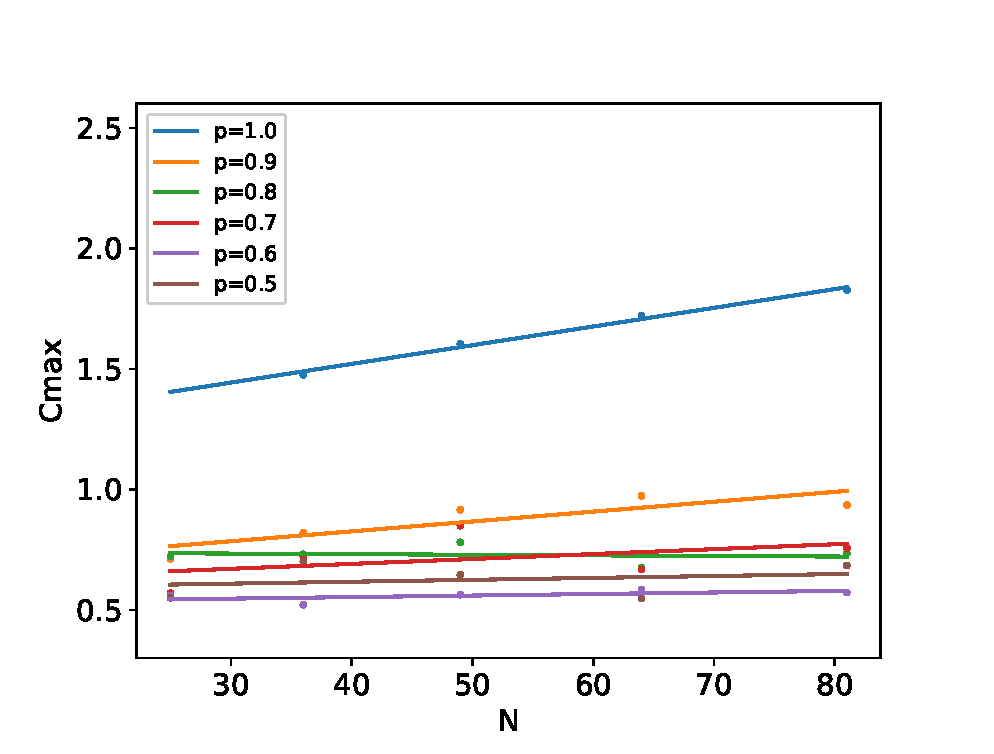
\includegraphics[width=0.8\linewidth]{Cmax(N)_scaling.eps}
	\caption{Расходимость теплоемкости в зависимости от количества  $N$ взаимодействующих спинов. На вкладке показаны значения $P_+$.}
	\label{fig:Cmax(N)_scaling}
\end{figure}

На рисунке \ref{fig:Cmax(N)_scaling} приводится зависимость максимального значения теплоемкости при критической температуре для различного количества $N$ взаимодействующих спинов. Наблюдаемый для $P_+>0.89$ рост максимального значения в поведении теплоемкости при критической температуре обычно называют расходимостью или сингулярностью. В данном случае при $P_+>0.89$ наличие расходимости в поведении теплоемкости системы взаимодействующих спинов обусловлено существованием фазового перехода второго рода. 

Отсутствие расходимости теплоемкости в интервале от $P_+>0.11$ до $P_+>0.89$ свидетельствует о существовании кроссовера, или конечной высоты пика в теплоемкости между фазой спинового стекла и фазой парамагнетика. Отсутствие сингулярности в поведении теплоемкости при переходе в фазу спинового стекла возможно связано с устройством статистической суммы, т.е пространством состояний, а именно с макроскопическим вырождением основного состояния для спиновых стекол. Для фрустрированных систем, к которым относятся спиновые стекла, существует макроскопическое вырождение основных состояний. Известно, что энтропия это своего рода ''скрытая теплота''. Поэтому при переходе в фазу спинового стекла при понижении температуры до критического значения уменьшение кинетической энергии движения спинов (уменьшение энергии термодинамических флуктуаций) не сопровождается ростом потенциальной энергии, которая упрочняет связи между спинами, как это имеет место в ферро- и антиферромагнетиках, а расходуется на образование возбуждений, или фрустраций. Для фрустрированных систем возбуждения сохраняются и в основных состояниях. 


При $P_+=0.0$ в антиферромагнетике и при $P_+=1.0$ в ферромагнетике существует только два основных состояния, фрустрации или возбуждения в которых отсутствуют. Например, для ферромагнетика при $T=0.0$ реализуется с одинаковой вероятностью состояние ''все спины --- вверх'', или состояние ''все спины --- вниз'', поэтому переход в эти основные состояния при понижении температуры приводит к резкому понижению свободной энергии, за счет резкого понижения энтропии (вырождения). Для конечных систем скачек изменения свободной энергии при переходе к основным состояниям будет не сильно выражен из-за больших значений вероятностей других состояний, поэтому и значения максимума в температурном поведении теплоемкости являются конечными. 


%Кроме того переход из состояний с отрицательным спиновым избытком к состоянию с положительным сопровождается преодолением потенциального барьера, что также требует увеличения времени наблюдения, которое растёт экспоненциально при уменьшении температуры, или при увеличении магнитного момента. Температура блокирования магнитного момента ''суперпарамагнитного кластера'' будет зависеть от объёма кластера, энергии анизотропии \cite{cullity2011, lubutin1997}. В реальных же системах, в том числе и в атомных кластерах, всегда существует, на ряду с энергией спин-спинового взаимодействия, энергия спин-орбитального взаимодействия, которая увеличивает потенциальный барьер, что приводит к отличной от нуля температуре, при которой может наблюдаться отличный от нуля ''заблокированный'' магнитный момент кластера \cite{lubutin1997, dietl2014, dmitriev2016}. В приведенных нами теоретических результатах температура имеет размерность обменных интегралов $J$.

%\textbf{Обнаружение системы ''суперпарамагнитного'' атомного кластера в одном из $2^{n-1}$ состоянии с отличном от нуля полным моментом возможно при уменьшении времени наблюдения системы, т.е. обнаружить систему в ферромагнитном состоянии.\cite{}}



\section{Перколяционные пороги и основное состояние}
В работе \cite{belokon2006} была приведена теоретическая магнитная фазовая диаграмма в осях критическая температура-концентрация ферромагнетика, где было показано, что согласуется с результатами \cite{newman2000efficient, jacobsen2014high, jacobsen2015critical}, что порог протекания по узлам квадратной решетки находится в пределах 0.591-0.593.

В настоящей работе представлена диаграмма $T(P_+)$, т.е. критические температуры для относительного количества ферромагнитных связей. Подтверждением достоверности теоретических оценок является, например, наблюдаемая при этом  расходимость температурного поведения теплоёмкости в области критической температуры в зависимости от числа спинов в системе. Точка наступления ферромагнетизма (антиферромагнетизма) легко обнаруживается по росту значения максимума теплоемкости для образцов различного $N$. Наши теоретические данные также согласуются с другими расчетами, см. например, точку Нишимори \cite{nishimori1980exact}, рисунок \ref{fig:Diag}. 

\begin{figure}[!ht]
	\centering
	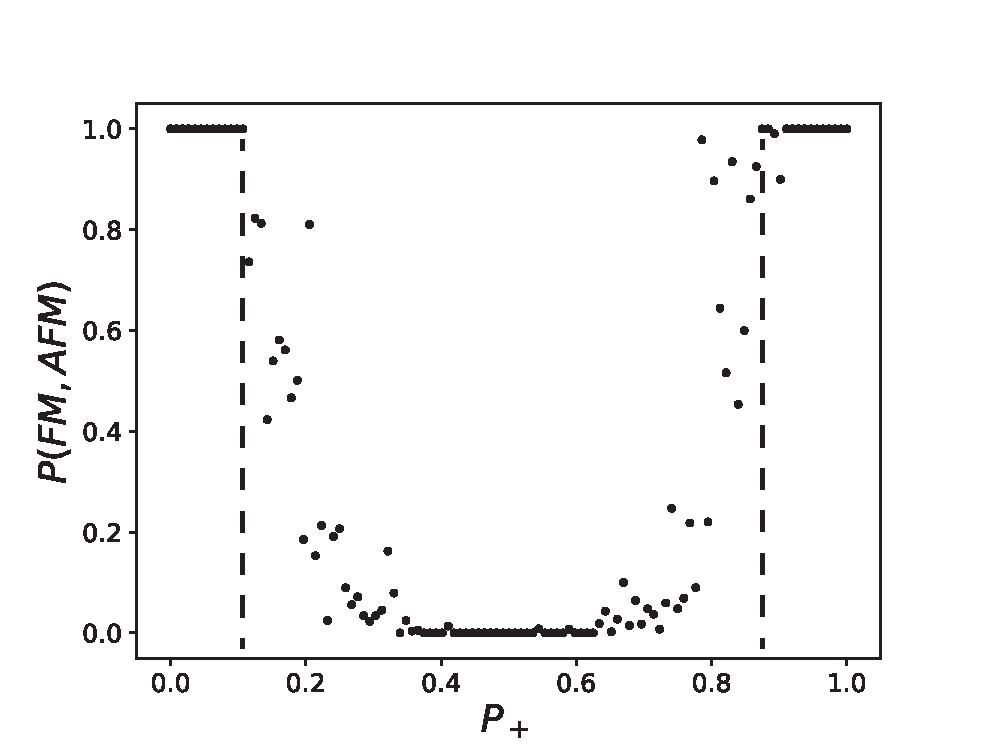
\includegraphics[width=0.8\linewidth]{Percolation.eps}
	\caption{Вероятность реализации перколяционного кластера спинов в основном состоянии, т.е. вероятность ферромагнетизма (антиферромагнетизма)}
	\label{fig:Percolation}
\end{figure}

Дополнительным теоретическим методом разделения фаз ферромагнетизма (антиферромагнетизма) и спинового стекла послужили численные расчеты перколяции спиновых кластеров, находящихся в основном состоянии. Для всех возможных конфигурации основного состояния каждого образца с фиксированным распределением обменных констант был произведен численный расчет. Вероятность появления кластера спинов основного состоянии такого, что он соединяет противоположные стороны образца, т.е. относительное число конфигураций основного состояния с наличием перколяции, в зависимости от распределения обменных констант, представлена на рисунке $\ref{fig:Percolation}$.  

Это позволяет легко различить фазы антиферромагнетизма и ферромагнетизма, наступающие при $H \rightarrow 0$ и $T \rightarrow 0$. Существует область концентрации $0.11<P_{+}<0.88$, характерной для спинового стекла, для которой у всех численно исследованных образцов наблюдаются мелкодисперсные кластеры в конфигурациях основного состояния, перколяционный кластер отсутствует.

\section{Фазовые переходы и кроссоверы в отличном от нуля внешнем магнитном поле.}

Строгое решение позволило построить теоретические магнитные фазовые диаграммы для плоской модели Изинга в отличном от нуля внешнем магнитном поле $T(P_{+},H)$. На рисунке \ref{fig:Diag1} представлена теоретическая магнитная фазовая диаграмма в магнитном поле $H=1.0$ в единицах $J$. Можно видеть наличие областей на фазовой диаграмме, в которых возможны переходы ''парамагнетик-спиновое стекло-ферромагнетик (ферромагнетик с наведенной намагниченностью)''  и ''парамагнетик-спиновое стекло-антиферромагнетик''. При этом на рисунке \ref{fig:Diag1} видно, что антиферромагнетик существует для $H=1.0$, что подтверждает не только расчет параметра фрустраций, но и температура Нееля, которая остается такой же, как при отсутствии внешнего магнитного поля.


\begin{figure}[!ht]
	\centering
	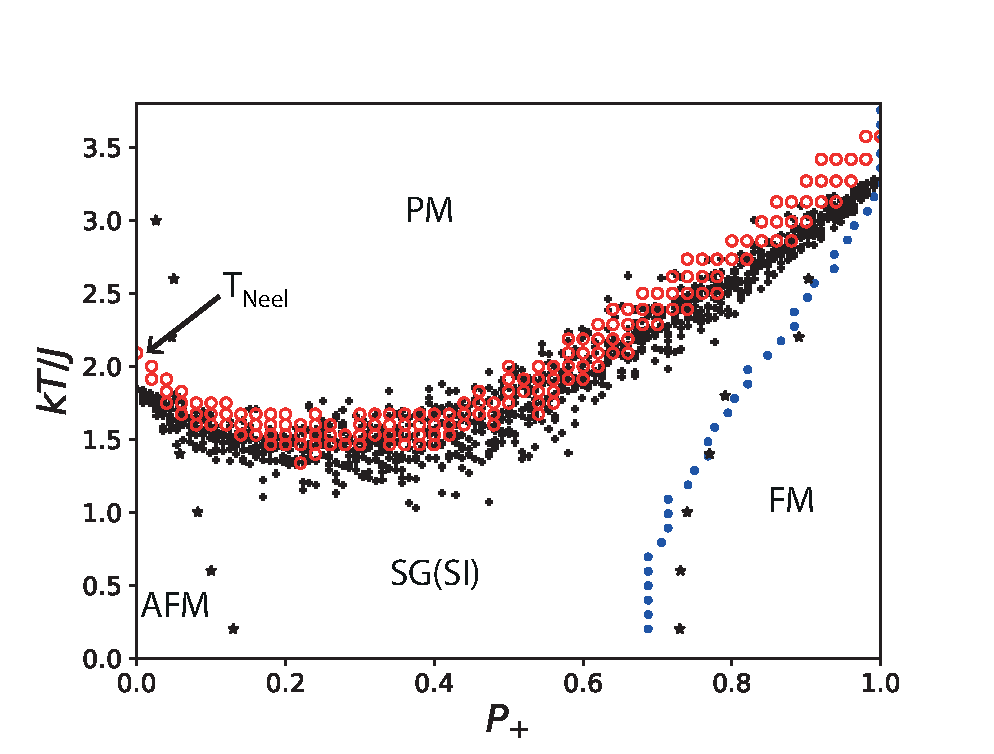
\includegraphics[width=0.8\linewidth]{Phase_diagram1_h1.0.eps}
	\caption{Фазовая диаграмма модели Изинга в поле $H = 1.0$.}
	\label{fig:Diag1}
\end{figure}

\begin{figure}[!ht]
	\centering
	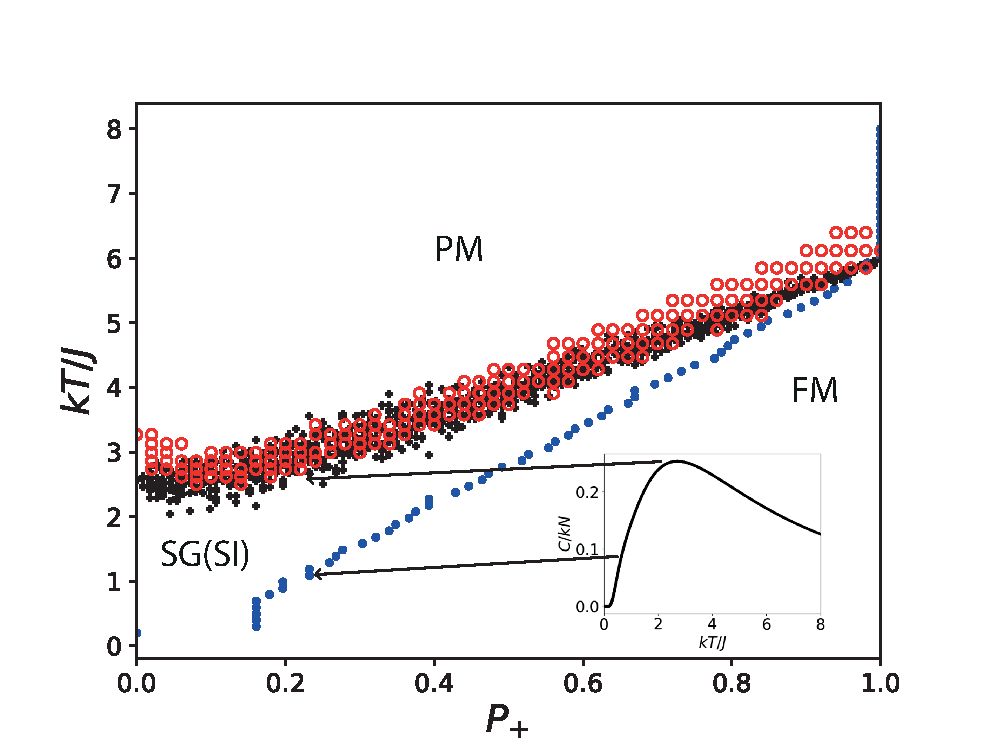
\includegraphics[width=0.8\linewidth]{Phase_diagram1_h4.0.eps}
	\caption{Фазовая диаграмма образцов в поле $H = 4.0$. На вкладке представлено температурное поведение теплоемкости $P_{+}=0.25$.}
	\label{fig:Diag4}
\end{figure}

Фазовая диаграмма в отличном от нуля относительно большом магнитном поле $H=4$ в единицах $J$ (рис. \ref{fig:Diag4}) позволяет заключить, что при увеличении модуля напряженности внешнего магнитного поля фаза антиферромагнетика подавляется полем. При этом состояние спинового стекла не исчезает бесследно. Расширяется область концентраций, для которой имеют место переходы ''парамагнетик-спиновое стекло-ферромагнетик''. В больших магнитных полях ошибка определения точки перегиба параметра фрустраций не позволяет использовать его для определения границы ферромагнитной фазы.  

Более высокая температура максимума теплоемкости для антиферромагнитной модели во внешнем магнитном поле по сравнению с $T_{Neel}$ свидетельствует о том, что произошло опрокидывание антиферромагнетика. На вкладке мы представили температурное поведение теплоемкости во внешнем магнитном поле для $P_+=0.25$. Никакой особенности теплоемкость не испытывает при переходе к возникновению наведенного ферромагнетизма.           % Глава 3
\chapter{Неэргодичность спинового стекла}\label{ch:ch4}

\section{Линии нестабильности}

\begin{figure}[!ht]
	\centering
	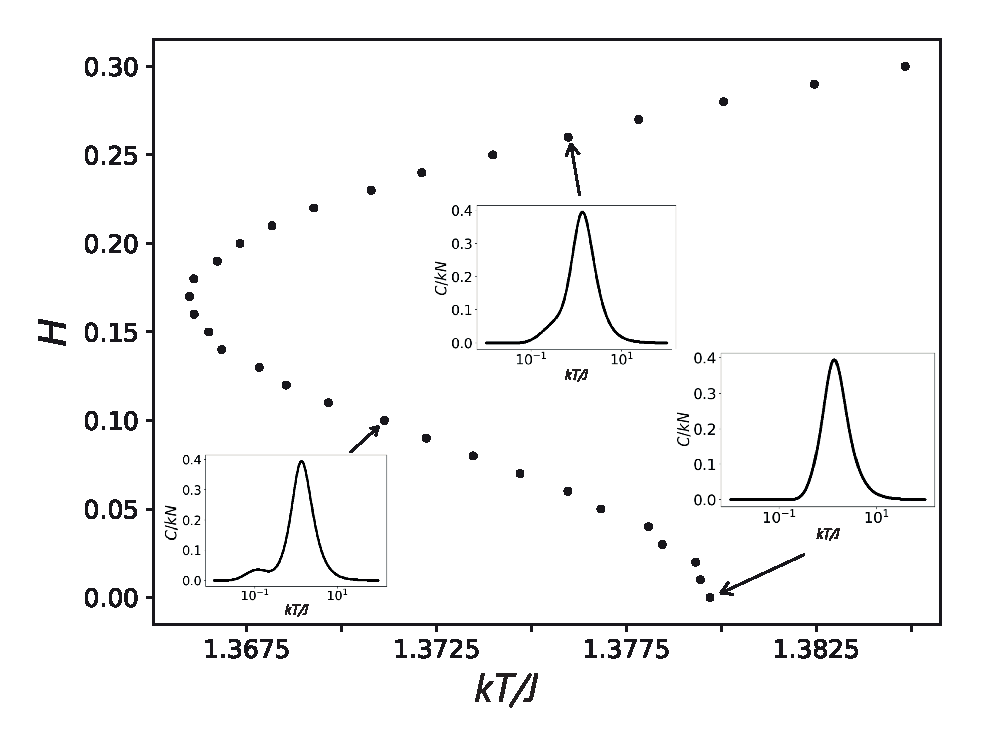
\includegraphics[width=0.8\linewidth]{Ginsburg_T_aver1.eps}
	\caption{Линия нестабильности системы конечного числа спинов Изинга в модели Эдвардса-Андерсона во внешнем магнитном поле. На вставках приводится температурное поведение теплоемкости во внешнем магнитном поле для систем $P_{+}=0.5$.}
	\label{fig:Stable_line}
\end{figure}

\begin{figure}[!ht]
	\centering
	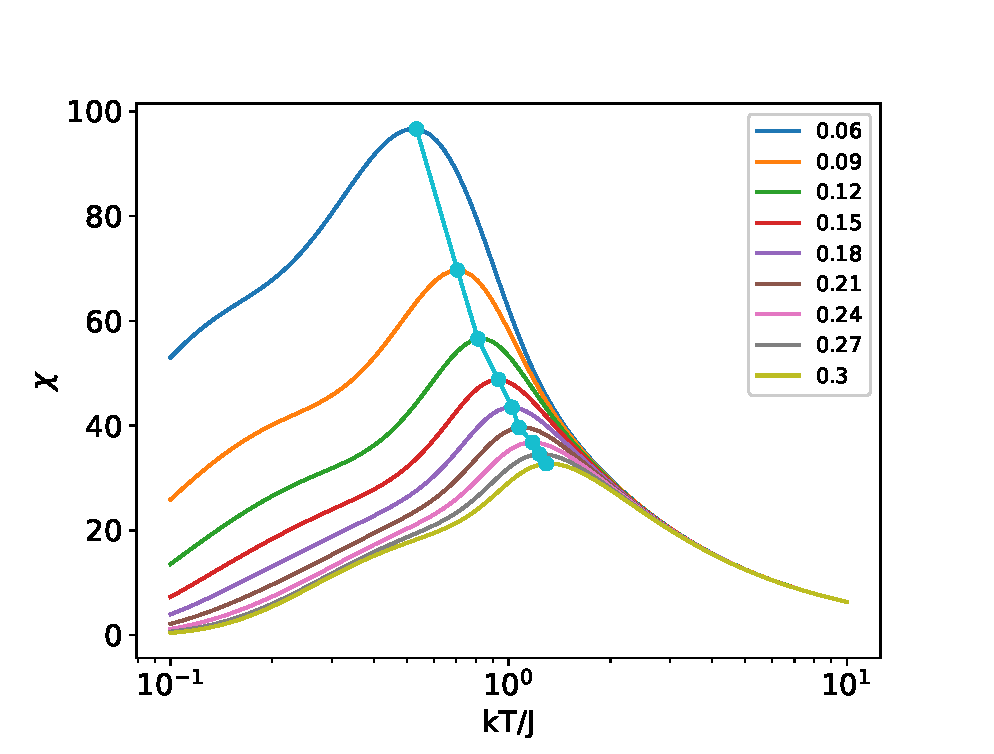
\includegraphics[width=0.8\linewidth]{Chi(kT)_J0_8.eps}
	\caption{Температурное поведение магнитной восприимчивости во внешнем магнитном поле для систем $P_{+}=0.5$ количеством частиц $N = 8 \times 8$. Значения модуля напряженности внешнего магнитного поля приведены на вкладке}
	\label{fig:Chi(kT)_J0_8.eps}
\end{figure}

Как отмечалось в работе \cite{takzei1984} на фазовой диаграмме $H-T$ можно наблюдать линию нестабильности Алмейды-Таулеса. В работе \cite{takzei1984} эти данные получены при анализе намагниченности при разных режимах проведения эксперимента. Наши результаты строгих вычислений показывают, что в малых полях наблюдается понижение средней температуры максимума теплоемкости с ростом малых значений внешнего магнитного поля $0.0<H<0.3$ в единицах обменных интегралов, см. рисунок \ref{fig:Stable_line}. Малыми мы считаем значения напряженности внешнего магнитного поля $H$ по отношению к напряженности полей взаимодействия между спинами. Небольшие изменения в низкотемпературном поведении теплоемкости возможно связаны с открытыми граничными условиями.


Данная линия получена по данным температурного поведения максимума теплоемкости. Данные по температурам максимумов теплоемкостей были усреднены по всем образцам с одинаковым $P_{+}$, в т.ч. на рисунках \ref{fig:Diag}, \ref{fig:Diag1} и \ref{fig:Diag4}. Оказалось, что для $P_{+}=0.5$ при увеличении модуля напряженности внешнего магнитного поля до $H<0.05$ в единицах $J$ температура максимума теплоемкости остается фиксированной. 

Можно предположить, что энергия Зеемана действует как хаотизирующий фактор, который приводит к понижению температуры максимума теплоемкости. В относительно высоких внешних магнитных полях $H>0.23$ температура максимума теплоемкости начинает расти, также, как в ферромагнитной модели из за эффекта опрокидывания спинового стекла.

Расчеты магнитной восприимчивости в поле произведены по формуле 
\begin{equation}
	\chi(T)=\frac{\partial \langle M \rangle (T)}{\partial T}\bigg|_{h\rightarrow 0}=\frac{\langle M^2 \rangle-\langle M \rangle ^2}{k T^2},
	\label{eq:ct}
\end{equation}
где
\begin{equation}
	\langle M \rangle (T) =\frac{1}{Z}\sum_{t=1}^{\Omega}g_t M_t \exp\left\{-\frac{E_t-h M_t}{kT}\right\}
	\label{eq:ct}
\end{equation}
и
\begin{equation}
	\langle M^2 \rangle (T) =\frac{1}{Z}\sum_{t=1}^{\Omega}g_t M_t^2 \exp\left\{-\frac{E_t-h M_t}{kT}\right\}.
	\label{eq:ct}
\end{equation}


На рисунке \ref{fig:Chi(kT)_J0_8.eps} видно, что при увеличении модуля напряженности внешнего магнитного поля температура максимума магнитной восприимчивости снижается для образов $P_+=0.5$. Таким образом, строгое вычисление статистической суммы   конечного числа спинов Изинга фактически означает, что физика изучаемых систем для $P_+=0.5$, которые находятся в состоянии спинового стекла является равновесной. Для объяснения существования линии нестабильности на $H-T$-диаграмме не требуется привлечения таких понятий как ''неэргодичность'', ''ультраметричность топологии пространства долин'', ''необратимость'' и других.           % Глава 4
\chapter*{Заключение}                       % Заголовок
\addcontentsline{toc}{chapter}{Заключение}  % Добавляем его в оглавление

%% Согласно ГОСТ Р 7.0.11-2011:
%% 5.3.3 В заключении диссертации излагают итоги выполненного исследования, рекомендации, перспективы дальнейшей разработки темы.
%% 9.2.3 В заключении автореферата диссертации излагают итоги данного исследования, рекомендации и перспективы дальнейшей разработки темы.
%% Поэтому имеет смысл сделать эту часть общей и загрузить из одного файла в автореферат и в диссертацию:

%Основные результаты работы заключаются в следующем.
%\input{common/concl}
%И какая-нибудь заключающая фраза.

Разработан алгоритм строгого расчета статистической суммы для конечного числа спинов Изинга на простой квадратной решетке со свободными граничными условиями для систем с $N=8\times8$ спинов. Строгий численный расчет позволил получить информацию о спиновых избытках конфигураций для фиксированных концентраций обменных констант в модели Изинга. Это позволило рассчитать модуль намагниченности, который в ферромагнитной модели Изинга был отличен от нуля для конечных температур.

Использован параметр фрустраций (\ref{eq:frustration_parameter}) для расчета критических температур перехода в антиферромагнитную и ферромагнитную фазы. Линейный рост параметра фрустраций в фазах ферромагнетика и антиферромагнетика обусловлен ростом числа возбуждений в основном и близких к основному низкоэнергетических состояниях. Переход в фазу спинового стекла в области точки перегиба приводит к выходу параметра фрустраций на насыщение. 

Исследование конфигураций основного состояния подтверждает, что параметр фрустраций выходит на насыщение при исчезновении перколяционного кластера. Дробление перколяционного кластера на мелкие кластеры увеличивает число возбуждений.

Переход в фазу спинового стекла из парамагнетика в отличном от нуля внешнем магнитном поле может быть определен по температуре максимума теплоемкости. Переход в фазу ферромагнетика из фазы спинового стекла происходит без видимых аномалий в температурном поведении теплоемкости при отличном от нуля внешнем поле (рис. \ref{fig:Stable_line}). Отсутствие аномалий в температурном поведении теплоемкости обусловлено тем, что фаза ферромагнетика является не спонтанной, а наведенной. Переход к наведенному ферромагнетизму контролируется энергией Зеемана. 

Проведенные численные эксперименты с помощью метода Метрополиса позволили получить температуры максимума теплоемкости в широком диапазоне значений обменных констант $P_+$, от антиферромагнитной области $P_+=0.0$, до ферромагнитной $P_+=1.0$. В области спинового стекла $P_+=0.5$ в отсутствии внешнего магнитного поля наблюдалось постоянство температур максимума теплоемкости и в точном решении, и в данных, полученных методом Монте-Карло, что может свидетельствовать об отсутствии эффекта количества частиц.

Понижение температуры максимума теплоемкости на $H-T$-диаграмме обусловлено увеличением термодинамической вероятности конфигураций с отличным от нуля спиновым избытком, т.е увеличением вклада энергии Зеемана в Гамильтониан.

Для ответа на вопрос о точном расчете критического значения обменной константы $P_+$ для фазовых переходов при $T\rightarrow0$ между состояниями ''$AFM-SG$'' и состояниями ''$FM-SG$'' необходимо исследование основных состояний. Однако, сегодня не существует каких либо подходов, схем или методов расчета, которые бы позволили разработать полиномиально-быстрые алгоритмы не только для поиска, но и для исследования статистических свойств основных состояний (энергии, вырождения, спинового избытка и других) даже в самой простой модели - модели Изинга произвольного распределения $J$. Сегодня отсутствует ответ на вопрос о возможном существовании способа расчета основного состояния в модели Изинга. Причина очевидна, основное состояние может быть получено только как точное решение. Любое приближение к основному состоянию позволяет получить только какое то из огромного множества возбужденных состояний. Важность исследования основных состояний обусловлена тем, что реализация основного состояния при $T\rightarrow0$ является достоверным событием.  Это состояние играет ключевую роль в термодинамике фазовых переходов.

Важные выводы в этой работе, на которых бы хотелось обратить внимание состоят в следующем. Первое --- линия нестабильности Алмейды-Таулеса не является следствием неравновесной физики или неэргодичности спинового стекла, поскольку выполнен строгий анализ всей статистической суммы, т.е. при бесконечном времени измерения.  Второе --- фазовая диаграмма была вычислена только с помощью компьютерных, вычислительных методов, алгоритмов исчерпывающего перечисления. Таким образом, компьютерные расчеты сегодня являются одним из важнейших инструментов теоретической физики для исследования существующих моделей, для которых строгое решение аналитическими методами пока не доступно.      % Заключение
\include{Dissertation/acronyms}        % Список сокращений и условных обозначений
\include{Dissertation/dictionary}      % Словарь терминов
\include{Dissertation/references}      % Список литературы
\include{Dissertation/lists}           % Списки таблиц и изображений (иллюстративный материал)

\setcounter{totalchapter}{\value{chapter}} % Подсчёт количества глав

%%% Настройки для приложений
\appendix
% Оформление заголовков приложений ближе к ГОСТ:
\setlength{\midchapskip}{20pt}
\renewcommand*{\afterchapternum}{\par\nobreak\vskip \midchapskip}
\renewcommand\thechapter{\Asbuk{chapter}} % Чтобы приложения русскими буквами нумеровались

\chapter{Программный код Glaurung}\label{app:A}

Листинг~\cref{lst:Glaurung_main} Представляет собой главный файл программы ,,Glaurung''. 

\begingroup
\captiondelim{ } % разделитель идентификатора с номером от наименования
\lstinputlisting[language={C},caption={main.cu},label={lst:Glaurung_main}]{listings/main.cu}
\endgroup

В листингах \cref{lst:Glaurung_cpuh, lst:Glaurung_gpuh} представлены заголовочные файлы для библиотеки функций центрального и графического процессоров

\begingroup
\captiondelim{ } % разделитель идентификатора с номером от наименования
\lstinputlisting[language={C},caption={cpu.h},label={lst:Glaurung_cpuh}]{listings/cpu.h}
\endgroup

\begingroup
\captiondelim{ } % разделитель идентификатора с номером от наименования
\lstinputlisting[language={C},caption={gpu.h},label={lst:Glaurung_gpuh}]{listings/gpu.h}
\endgroup\texttt{}

Листинги \cref{lst:Glaurung_cpucpp, lst:Glaurung_gpucu} содержат реализации функций для центрального и графического процессоров

\begingroup
\captiondelim{ } % разделитель идентификатора с номером от наименования
\lstinputlisting[language={C},caption={cpu.h},label={lst:Glaurung_cpucpp}]{listings/cpu.cpp}
\endgroup

\begingroup
\captiondelim{ } % разделитель идентификатора с номером от наименования
\lstinputlisting[language={C},caption={gpu.h},label={lst:Glaurung_gpucu}]{listings/gpu.cu}
\endgroup\texttt{}
        % Приложения

\setcounter{totalappendix}{\value{chapter}} % Подсчёт количества приложений

\end{document}
